\chapter{\IfLanguageName{dutch}{De opstelling en testmethodologie}{The Setup and Testing Methodology}}%
\label{ch:basisopstelling}

\section{Inleiding}

De opstelling is ontworpen met het oog op het evalueren en vergelijken van netwerkprestaties over wifi, 4G en privaat 5G binnen de context van gebouwbeheersystemen, meer bepaald voor toepassingen in verlichting en HVAC-sturing.
Aangezien de focus in eerste instantie ligt op netwerkanalyse, wordt gekozen voor een flexibele en programmeerbare testomgeving. In plaats van de oorspronkelijk gekozen Schneider Electric SpaceLogic SmartX AS-P controller, die niet beschikbaar bleek in HOGENT, wordt een Raspberry Pi gebruikt als centrale testnode.


De Raspberry Pi simuleert de rol van een AS-P controller, voert netwerkmetingen uit, en zorgt voor communicatie met het netwerk. De meetopstelling is opgebouwd rond een industriële RUTX50-router, die in staat is om zowel 4G als 5G-connectiviteit aan te bieden. Zowel de Raspberry Pi als een pc zijn bekabeld verbonden met de router voor een maximale stabiliteit van de interne netwerkkoppeling.

\begin{figure}
    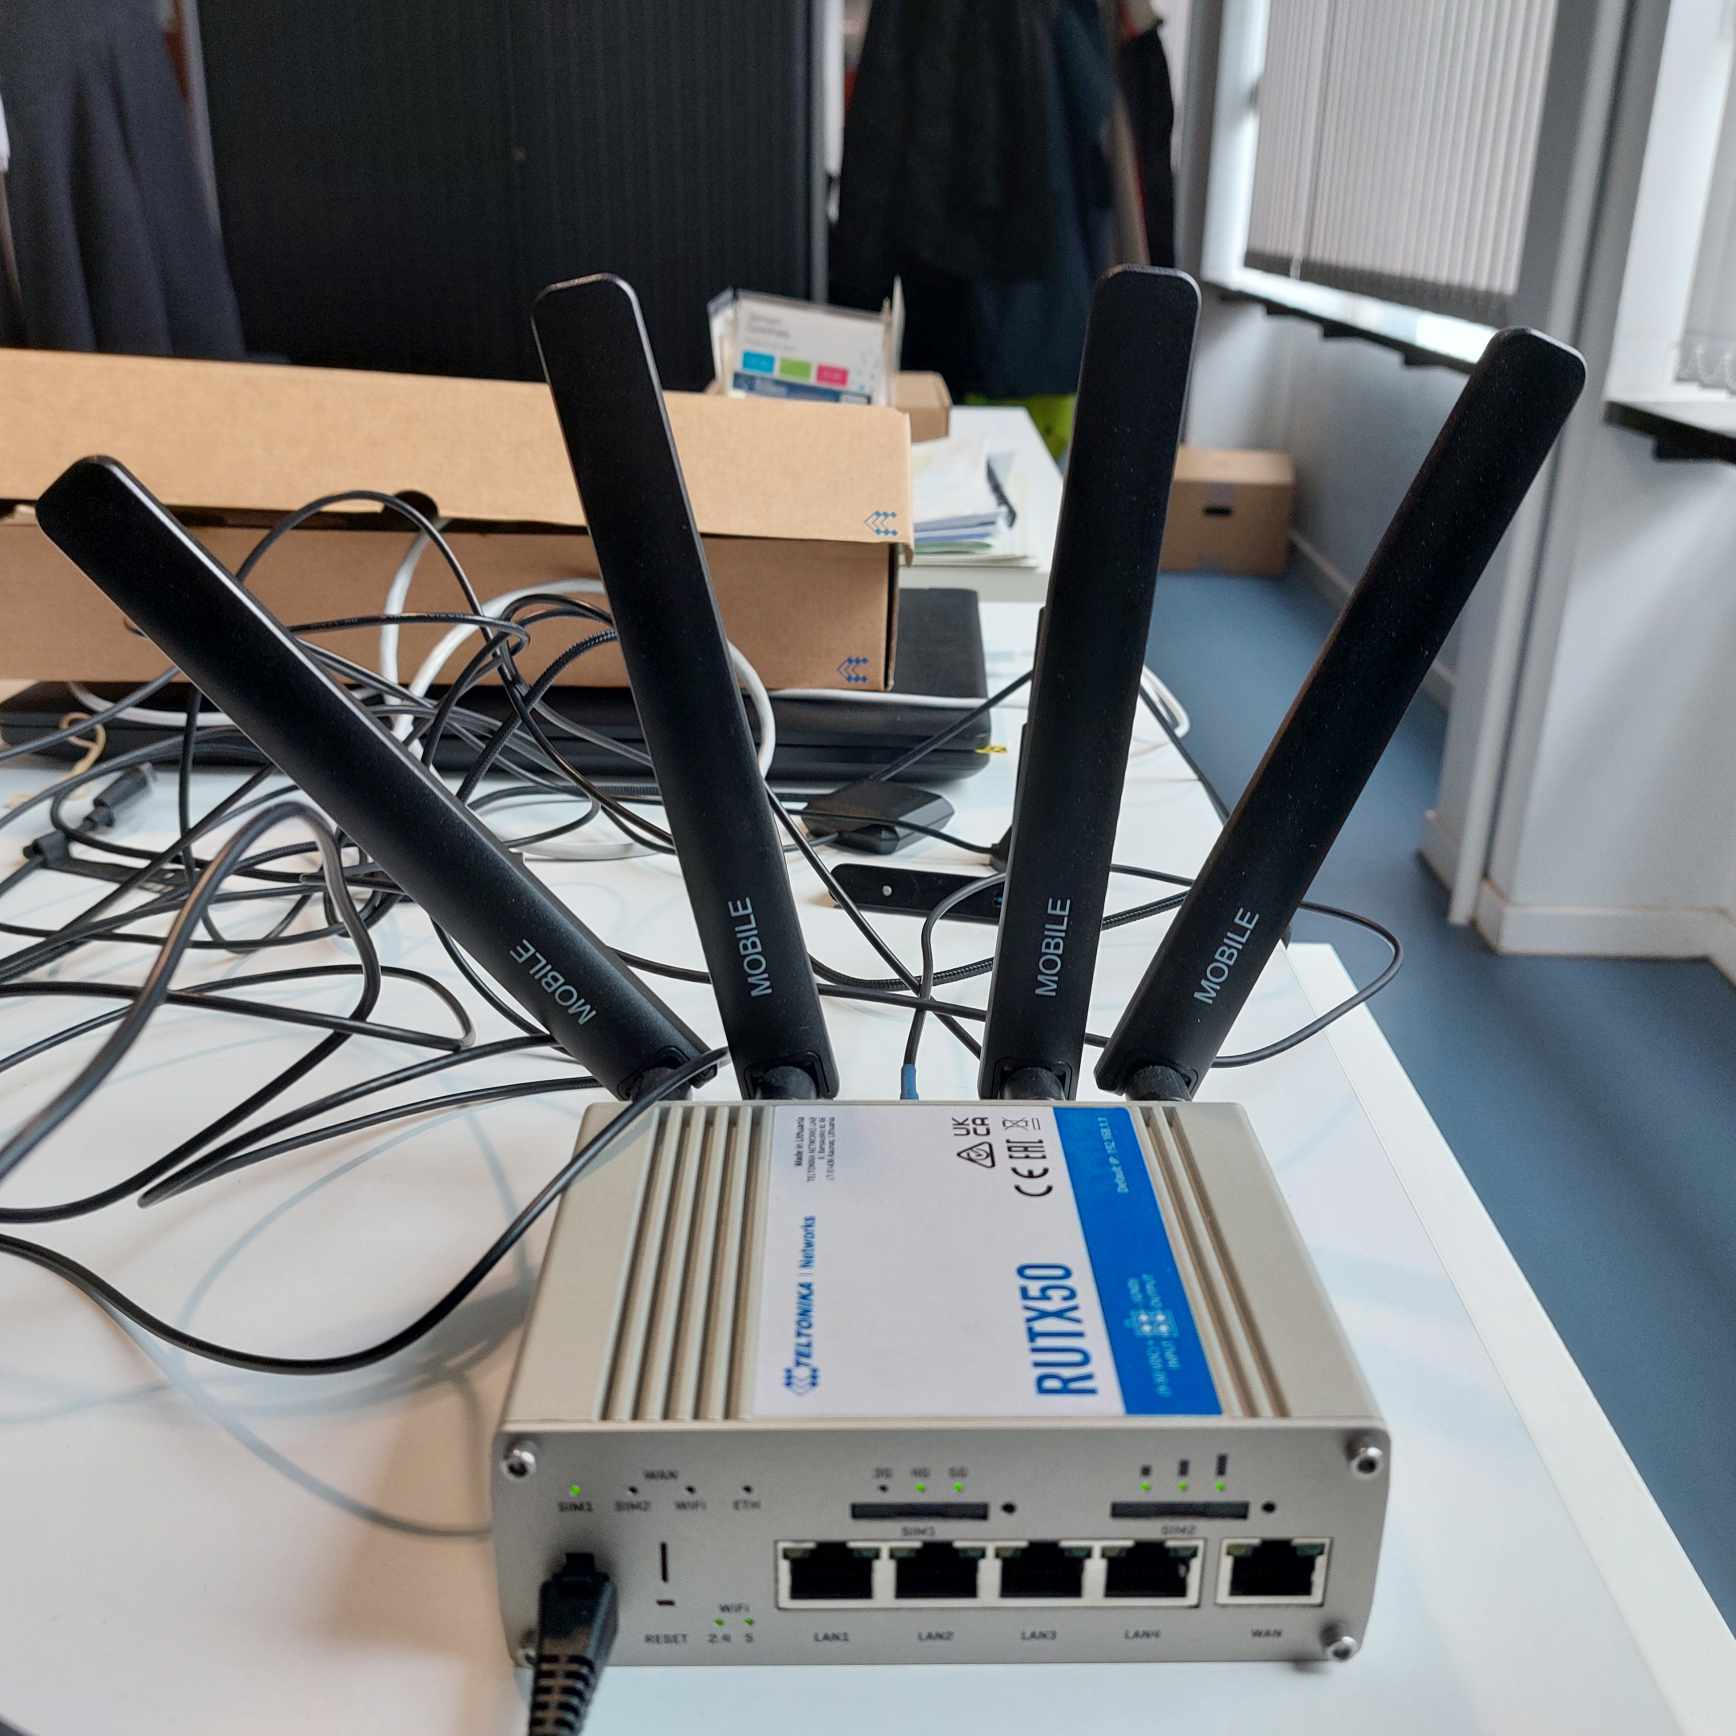
\includegraphics[width=0.8\textwidth]{../graphics/RUTX50.jpg}
    \caption[router]{\label{fig:router}info bij fig}
\end{figure}

\section{Motivatie voor gebruik van de Raspberry Pi}

De Raspberry Pi biedt in deze meetcontext meerdere voordelen. Ten eerste heeft het platform een hoge flexibiliteit, aangezien het ondersteuning biedt voor meerdere programmeertalen en bibliotheken. Voorbeelden daarvan zijn Python, bash, iperf3 en speedtest-cli. Daarnaast is met de Raspberry Pi een verregaande automatisatie mogelijk. Dit laat toe om complexe testreeksen op een automatische en herhaalbare manier uit te voeren. Tot slot is het een zeer compact toestel waardoor het zeer makkelijk als mobiele meetnode kan worden ingezet in uiteenlopende netwerkomgevingen.

\begin{figure}
    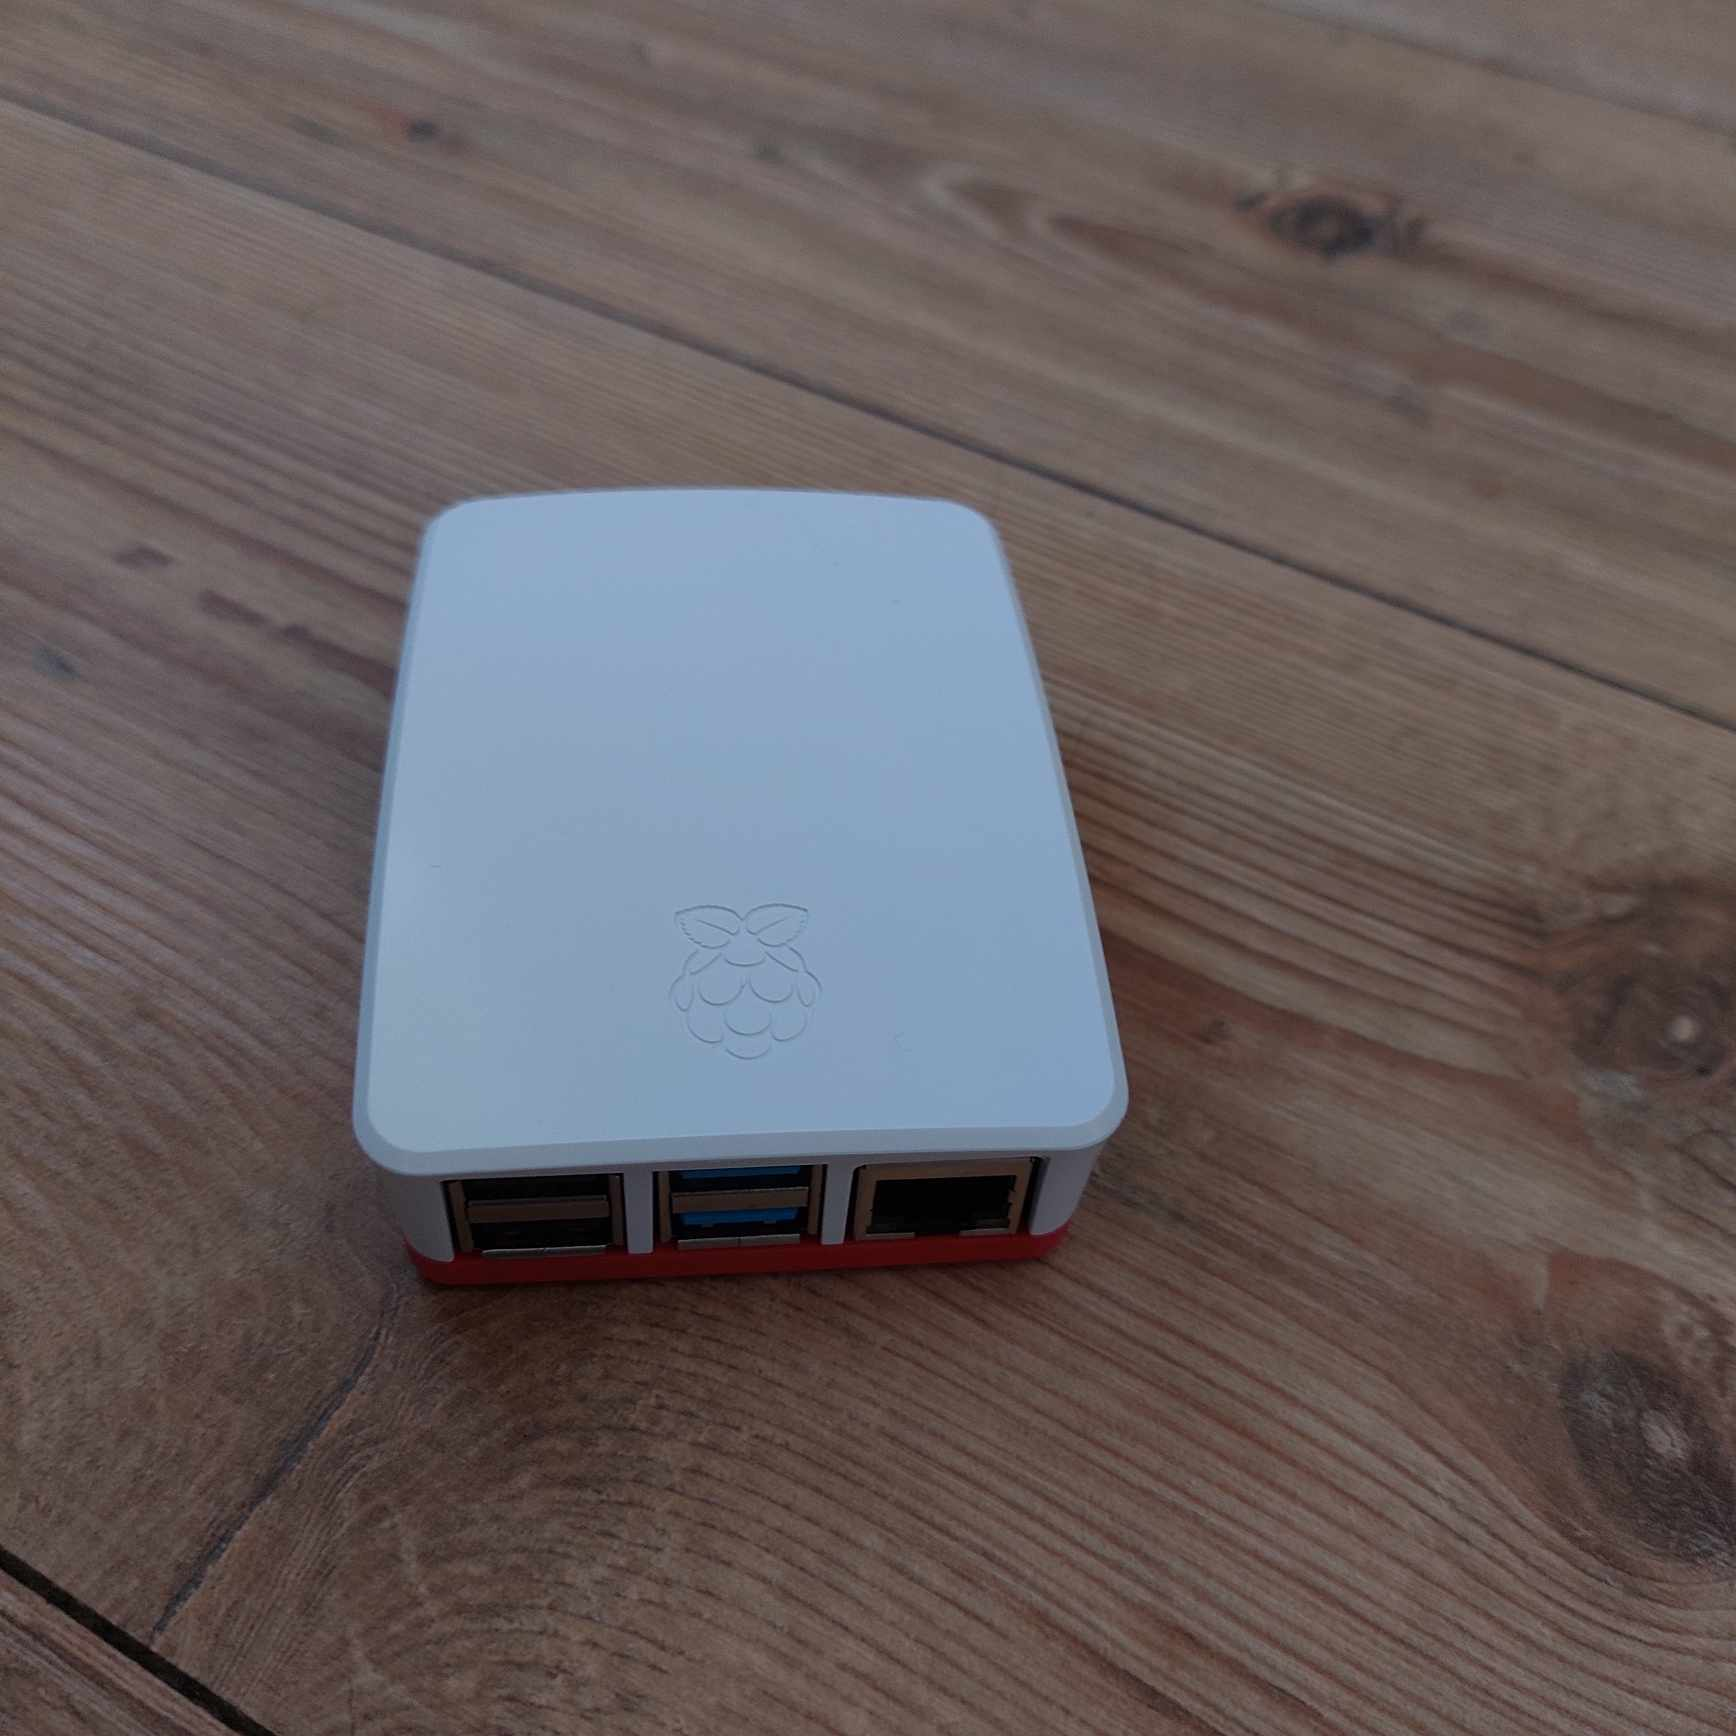
\includegraphics[width=0.8\textwidth]{../graphics/Rasberry_pi.jpg}
    \caption[rasberry pi]{\label{fig:rasberrypi}info bij fig}
\end{figure}

\section{Overzicht van de meetopstelling}

\begin{figure}
    
    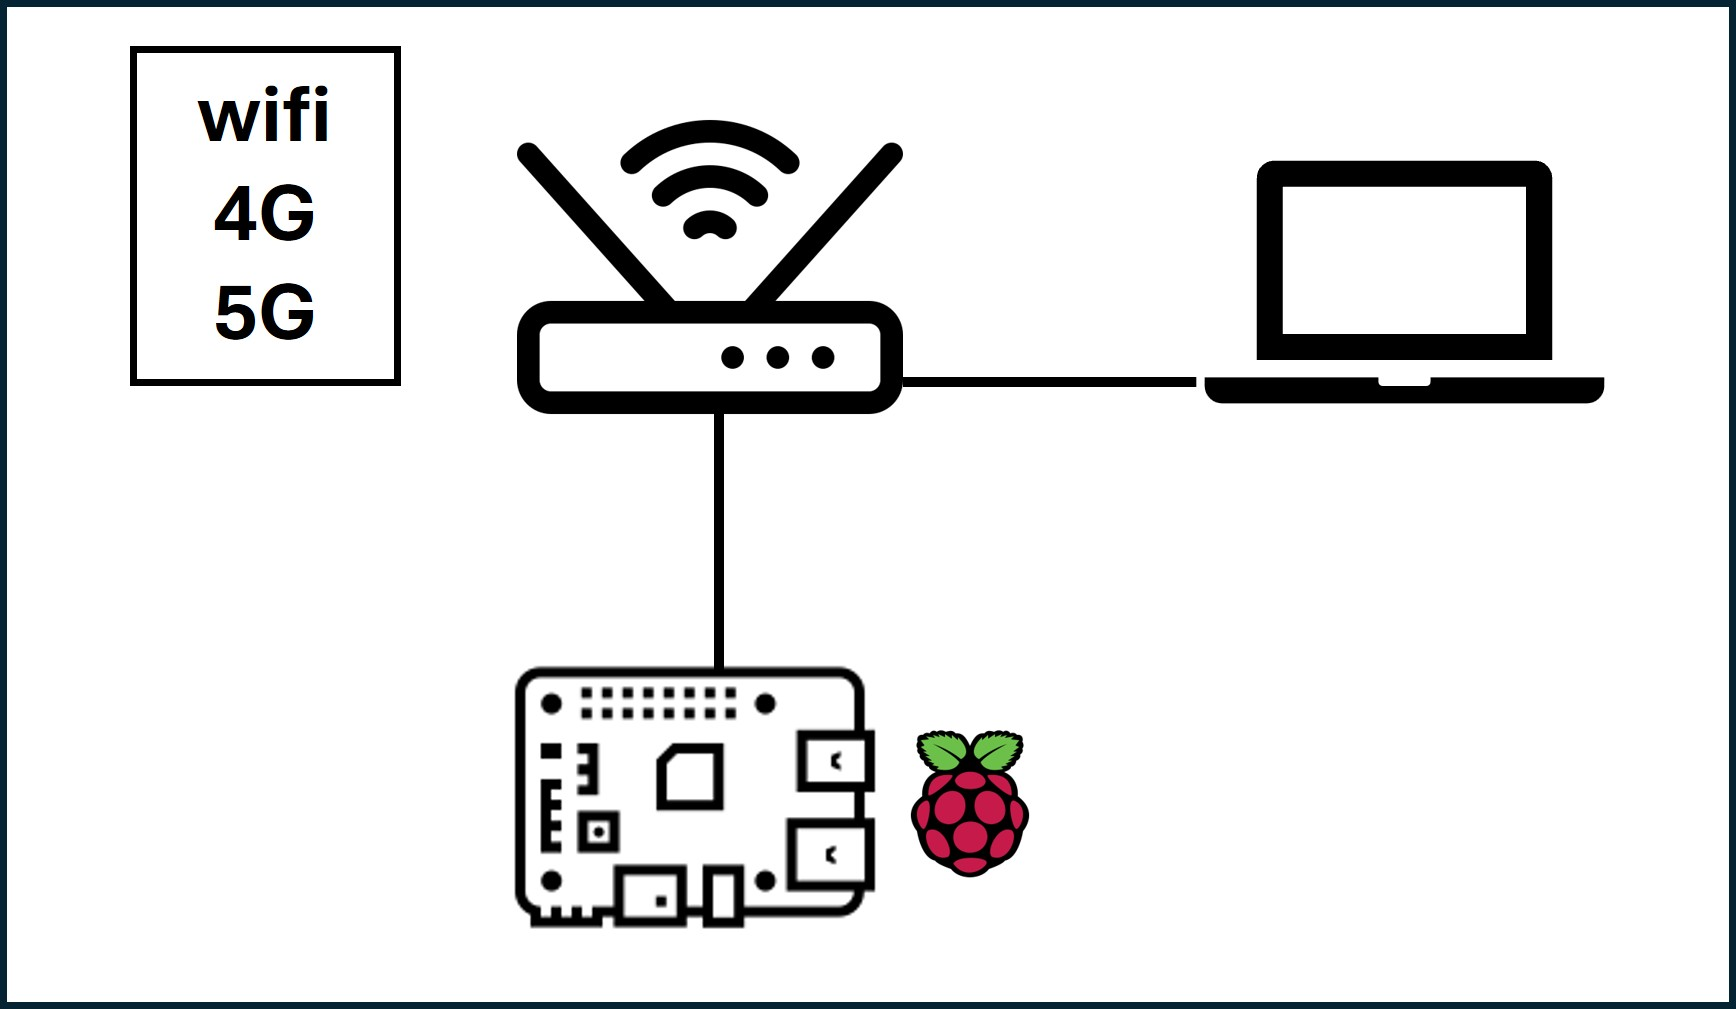
\includegraphics[width=0.8\textwidth]{../graphics/Opstelling_1.jpg}
    \caption[opstelling 1]{\label{fig:opstellingpi}info bij fig}
\end{figure}
\begin{itemize}
    \item De Raspberry Pi en de Windows-pc zijn bekabeld verbonden met een RUTX50-router.
    \item Deze router biedt afwisselend connectiviteit via 4G, publiek 5G en privaat 5G (afhankelijk van de testomgeving).
    \item Op de Raspberry Pi worden diverse scripts uitgevoerd die netwerkparameters meten zoals latency, jitter, throughput, packet loss, en responsiviteit.
    \item De pc fungeert als referentiepunt voor iperf3-sessies en host ook een lokale HTTPS-endpoint via een Python-API.
\end{itemize}

Voor de uitvoering van de testen werd de Raspberry Pi voorbereid met een actuele versie van Raspberry Pi OS (Lite), waarop de nodige tools geïnstalleerd werden zoals ping, iperf3, curl en Node-RED. Deze werden geïnstalleerd via het pakketbeheer apt met commando’s zoals \textbf{sudo apt install iperf3 curl}, terwijl Node-RED werd toegevoegd via het officiële installatie­script van Node-RED.

\section{Beschrijving van de uitgevoerde testen}

\subsection{Pingtest (latency en packet loss)}
Het ping-commando meet de netwerkprestaties van de Raspberry Pi binnen verschillende netwerkomstandigheden. Het doel van deze meting is om de gemiddelde latency (Round-Trip Time, RTT), het aantal verloren pakketten en de spreiding in vertraging (minimum en maximum RTT) tussen de Raspberry Pi en een extern internetadres (in dit geval het publieke DNS-adres van Google, 8.8.8.8) in kaart te brengen.

Het gebruikte commando is als volgt: \textbf{ping -c 250 8.8.8.8 > ping*.log}

\begin{itemize}
    \item In dit commando staat ’-c 250’ voor het aantal echo-verzoeken dat naar het opgegeven IP-adres wordt gestuurd, in dit geval worden er dus 250 ICMP-pakketten verzonden. 
    \item De output van het commando wordt omgeleid naar een logbestand met de naam ping*.log, waarin * verwijst naar een unieke identificatie per testreeks (bijvoorbeeld: ping4g1.log).
\end{itemize}


De metingen worden vier keer uitgevoerd per netwerkmodus zowel voor wifi als voor 4G als voor 5G waardoor er per technologie in totaal 1000 individuele metingen beschikbaar zijn. Deze opzet maakt het mogelijk om statistisch relevante conclusies te trekken over de prestaties van elk netwerk.
De belangrijkste doelvariabelen die uit deze metingen worden afgeleid, zijn de gemiddelde latency, het minimum en maximum van de Round-Trip Time (RTT), en het percentage pakketverlies. Deze variabelen geven samen een beeld van de stabiliteit en efficiëntie van de netwerkverbinding onder verschillende omstandigheden.


\subsection{TCP throughputtest (bandbreedte en betrouwbaarheid)}
De troughputtest bepaalt de netto datadoorvoer en de stabiliteit van de Transmission Control Protocol (TCP)-verbinding tussen de Raspberry Pi en de externe Windows-pc. De metingen worden uitgevoerd met behulp van de tool iperf3, specifiek ontworpen voor performantie-evaluaties van netwerkverbindingen. 
De testopstelling vereist dat de iperf3-server op de ontvangende pc wordt geactiveerd. Download iperf3 voor Windows via: ’https://iperf.fr/iperf-download.php’.
De server wordt dan gestart via het volgende commando: \textbf{iperf3.exe -s} 

Zodra de server actief is, wordt de Raspberry Pi als client gebruikt en voert deze het volgende commando uit: \textbf{iperf3 -c [PC-IP] -t 120 > iperf*.log}

\begin{itemize}
    \item In dit commando vervangt [PC-IP] het IP-adres van de pc waarop de server draait.
    \item De vlag -t 120 specificeert dat de meting gedurende 120 seconden (twee minuten) wordt uitgevoerd. 
    \item De uitvoer wordt opgeslagen in een logbestand met een herkenbare naam (iperf*.log), waarbij * verwijst naar de specifieke testomstandigheden.
\end{itemize}


Voor elke netwerkomgeving 4G en 5G worden vier aparte sessies uitgevoerd, telkens met een duur van twee minuten. Dit zorgt voor een voldoende representatieve steekproef om statistische vergelijkingen mogelijk te maken. 
De variabelen voor de analyse zijn de doorvoersnelheid per seconde, de variatie in die snelheden over de volledige sessie (als maat voor stabiliteit), en het aantal eventuele TCP-retransmissies (die een indicatie geven van de  netwerkbetrouwbaarheid en congestie). Deze parameters geven inzicht in de prestaties van het TCP-protocol onder reële omstandigheden.

\subsection{UDP jittertest}
Om de eigenschappen van een niet-verbindingsgerichte netwerkoverdracht te analyseren, wordt een meting uitgevoerd met het User Datagram Protocol (UDP). In tegenstelling tot TCP, biedt UDP geen garantie op levering of volgorde van data, waardoor deze test specifiek gericht is op het bepalen van jitter (variatie in vertraging tussen opeenvolgende pakketten) en het aantal verloren pakketten


De meting wordt uitgevoerd met behulp van iperf3, waarbij de Raspberry Pi als client fungeert en een pc met actieve iperf3-server als ontvanger. Het volgende commando wordt op de Raspberry Pi gebruikt: \textbf{iperf3 -c [PC-IP] -u -b xM -t 120 > iperfudp*.log}

\begin{itemize}
    \item In dit commando specificeert de vlag -u dat het om een UDP-verbinding gaat. 
    \item Met -b xM wordt de bandbreedte vastgelegd op x megabit(s) per seconde waarbij x de waardes 1, 5 en 50 heeft.
    \item De testduur wordt ingesteld op 120 seconden via -t 120, en de uitvoer wordt gelogd in een bestand genaamd iperfudp*.log, waarbij * een placeholder is voor de testconfiguratie of het sessienummer. 
    \item Het IP-adres van de pc-server moet worden ingevuld op de plaats van [PC-IP].
\end{itemize}


De test wordt viermaal herhaald per netwerkomgeving, wat een voldoende grote dataset oplevert om verschillen tussen technologieën te kunnen detecteren. 
Tijdens de analyse worden drie hoofdparameters geëvalueerd: de jitter, het absolute aantal verloren pakketten, en de verhouding van verloren tot totaal verzonden pakketten (lost/total ratio). Deze meetwaarden geven inzicht in de betrouwbaarheid en stabiliteit van de UDP-verbinding, en zijn belangrijk bij het beoordelen van de geschiktheid van een netwerk voor latencygevoelige toepassingen.



\subsection{Speedtest via Node-RED}
Node-RED is een visueel programmeerplatform dat vaak wordt ingezet binnen IoT-toepassingen voor het beheren van datastromen tussen sensoren, servers en applicaties. Het doel van deze meting is het evalueren van de download- en uploadsnelheden binnen een realistische en visuele omgeving. 
Node-RED wordt lokaal opgestart op de Raspberry Pi met het commando node-red. De gebruikersinterface van Node-RED is toegankelijk via het interne IP-adres van de Pi op poort 1880, bijvoorbeeld via: ’http://[IP-Pi]:1880’
De gebruikte flow, weergegeven in Figuur~\ref{fig:nodered-flow}, bestaat uit drie knooppunten: een inject-node (timestamp), een exec-node met een curl-commando, en een debug-node. 

Bij activatie verstuurt het systeem via curl een HTTP POST-verzoek naar een endpoint op de pc: \textbf{curl -k -X POST http://192.168.1.40:8080 -d ’”value”: 42’ -H ”Content-Type: application/json”}


\begin{itemize}
    \item Hierbij staat -k toe dat een onveilige (zelfondertekende) verbinding wordt geaccepteerd
    \item -X POST specificeert het HTTP-methodetype
    \item de data wordt in JSON-formaat verstuurd met de correcte content header.
\end{itemize}

Deze opzet bootst realistische API-interacties na, zoals ze vaak voorkomen in IoT-systemen waarbij sensorgegevens of statussen naar een centrale dienst worden gepusht.


\begin{figure}[h]
    \centering
    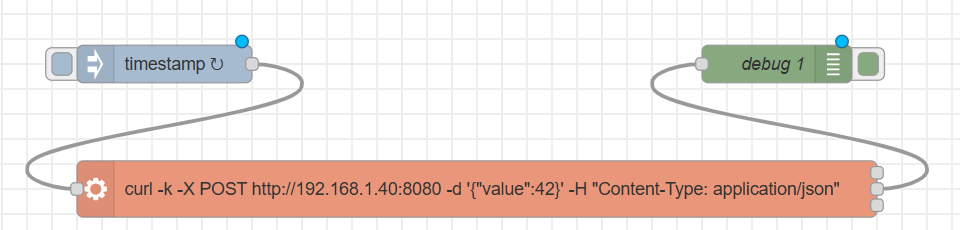
\includegraphics[width=0.9\textwidth]{../graphics/node-red_flow.png}
    \caption{Node-RED-flow voor het verzenden van HTTP POST-verzoeken naar een externe endpoint.}
    \label{fig:nodered-flow}
\end{figure}

\subsection{Smart verlichting test}
Het doel van deze meting is het evalueren van de betrouwbaarheid en de reactietijd van een eenvoudige IoT-toepassing als smart verlichting bij verschillende onderliggende netwerkverbindingen.
Hierbij wordt specifiek onderzocht in welke mate de netwerktechnologie (wifi, 4G en 5G) de snelheid en betrouwbaarheid van een commando van een gebruiker naar een slim toestel beïnvloed.
In plaats van de Raspberry Pi wordt in deze testopstelling een Philips Hue Bridge gebruikt als edgecontroller. Deze wordt verbonden met het netwerk via een bekabelde ethernetverbinding. Een slimme lamp die via deze bridge wordt aangestuurd, fungeert als uitvoerend toestel.

\begin{figure}
    
    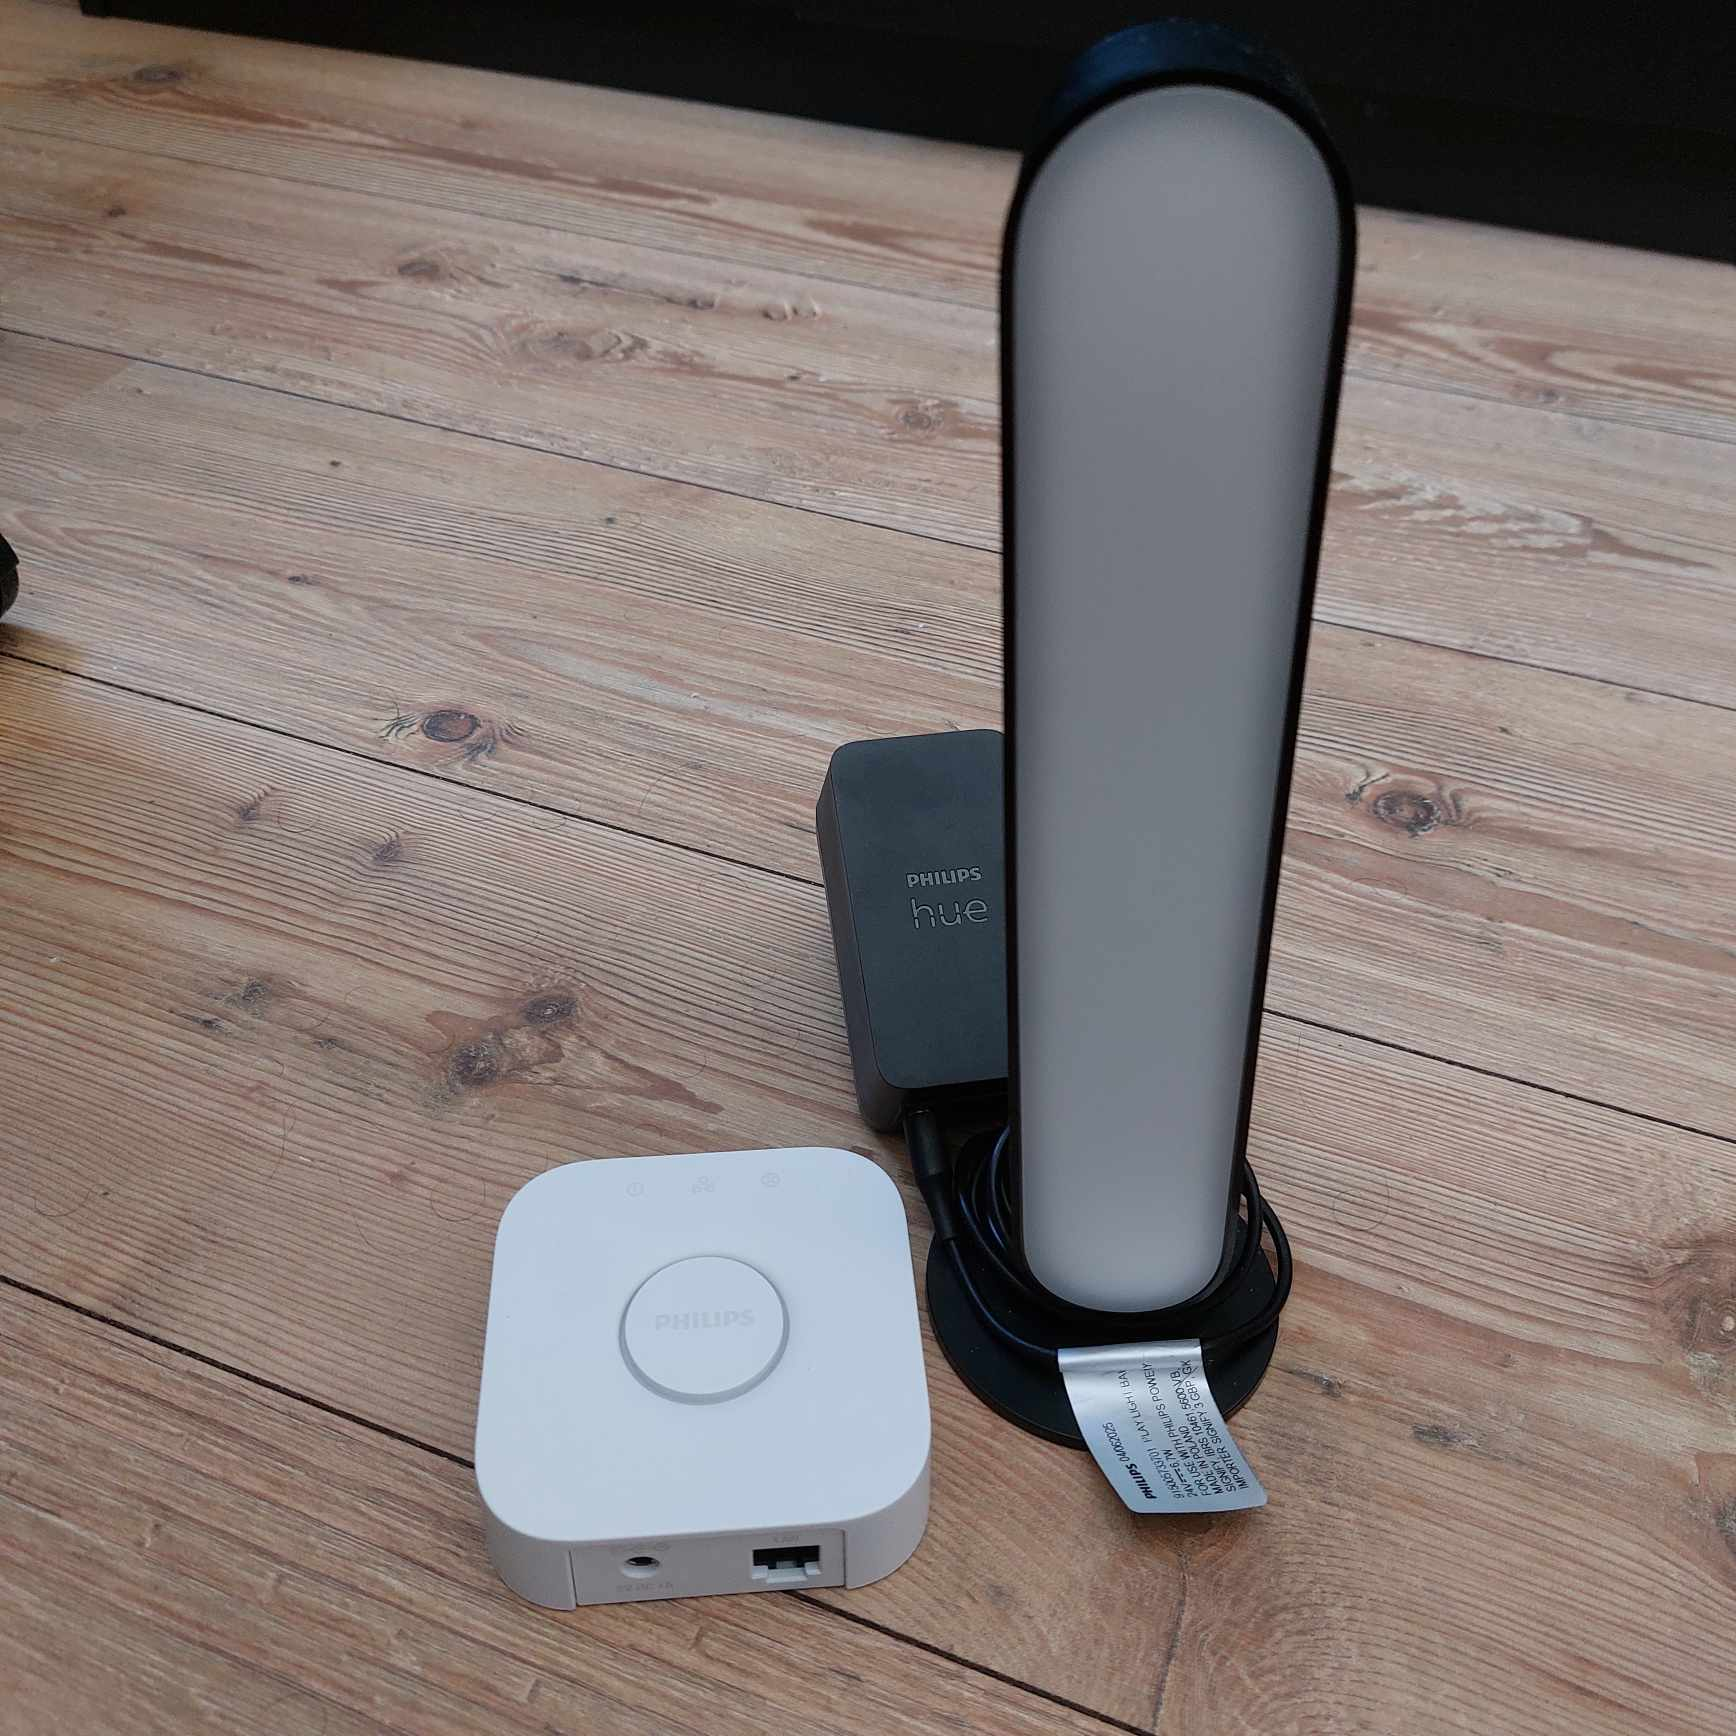
\includegraphics[width=0.8\textwidth]{../graphics/philips_hue.jpg}
    \caption[philips hue hardware]{\label{fig:philips}info bij fig}
\end{figure}
\begin{figure}
    
    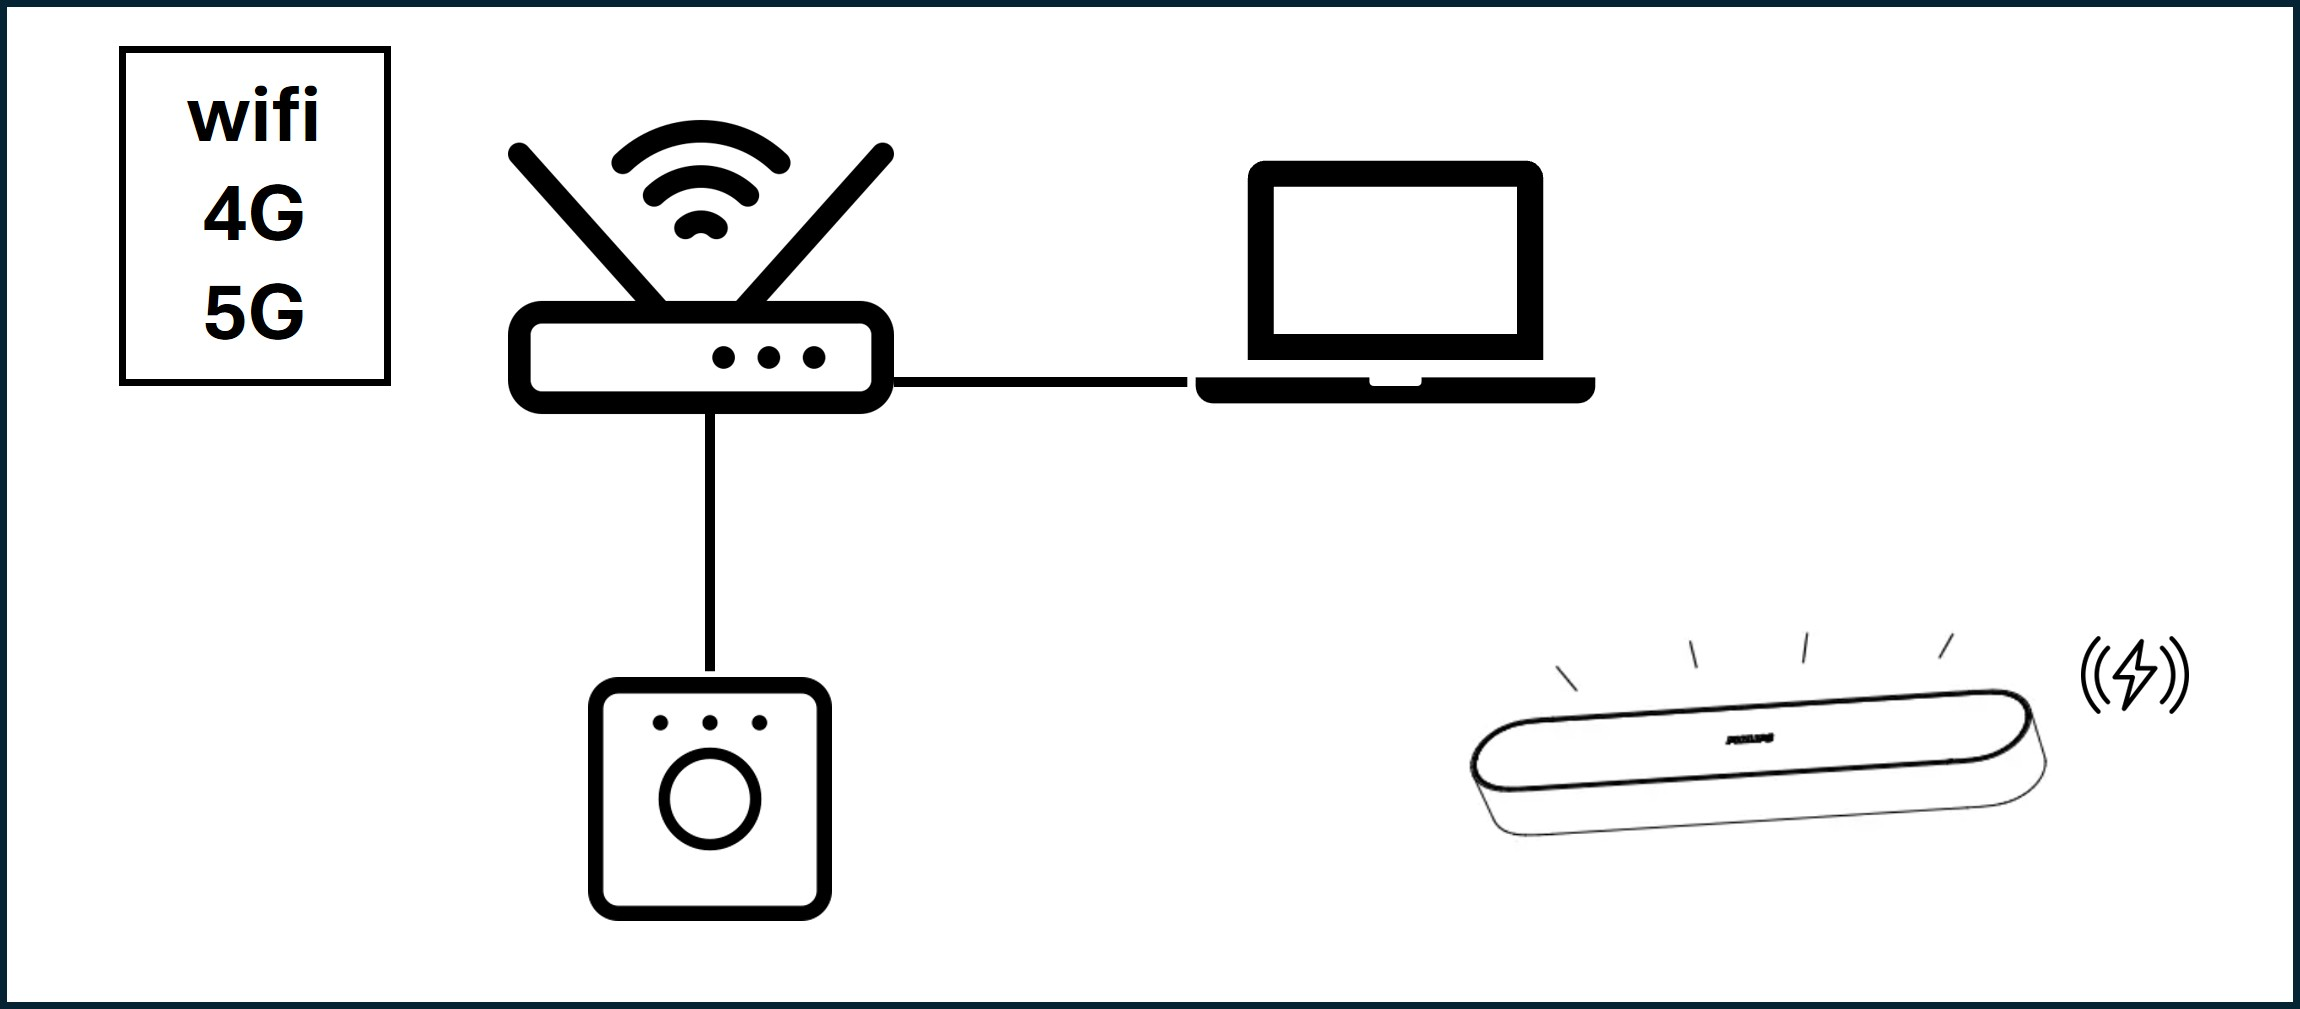
\includegraphics[width=0.8\textwidth]{../graphics/Opstelling_2.jpg}
    \caption[philips opstelling]{\label{fig:opstellingphilips}info bij fig}
\end{figure}
Het centrale testscript, lichtscript.py (zie bijlage \ref{script}), is geschreven in Python en maakt gebruik van de Hue API. Het script voert bij elke iteratie twee opeenvolgende toggle-operaties uit (aan-uit of uit-aan) op de lamp. Voor elke uitvoering wordt gelogd wat de reactiesnelheid is en of deze succesvol is.



De kernparameter die gemeten wordt, is de totale tijd tussen het initiëren van het commando en het effectief voltooien van de toggle-operatie. Eventuele fouten (bv. timeouts of mislukte requests) worden eveneens geregistreerd als indicatoren van netwerkbetrouwbaarheid.
De test wordt uitgevoerd op de 3 netwerken. Per netwerk worden 100 iteraties uitgevoerd van het script, met telkens twee toggles per iteratie. Dit resulteert in 200 metingen per script en 400 metingen in totaal per netwerk.
Deze experimentele opzet laat toe om te evalueren hoe netwerkvertragingen en -stabiliteit impact hebben op de werking van een eenvoudige maar representatieve IoT-toepassing. De resultaten geven inzichten voor het gebruik van mobiele netwerken in real-time of near-real-time besturingssystemen binnen smart building-contexten (smart building concepten).



\section{Samenvatting van meetdoelen}

Het opgezette testkader van deze bachelorproef was ontworpen om onderbouwde antwoorden te formuleren op de centrale onderzoeksvraag en de bijbehorende deelvragen over het gebruik van mobiele netwerken in gebouwbeheersystemen. Daarbij werd een combinatie van netwerkprestatietesten en functionele toepassingstesten ingezet om zowel kwantitatieve als kwalitatieve data te verzamelen.

De eerste onderzoeksvraag betrof de objectieve vergelijking van netwerkparameters: \textit{Wat is het verschil in latency, jitter, packet loss en throughput tussen 4G, wifi en privaat 5G?} Deze parameters werden nauwkeurig gemeten via tools als \texttt{ping}, \texttt{iperf3} en \texttt{speedtest-cli}, uitgevoerd in zo identiek mogelijke testomstandigheden. De tweede onderzoeksvraag richtte zich op de betrouwbaarheid van netwerken bij functionele toepassingen binnen een smart building: \textit{Hoe betrouwbaar verlopen netwerkverzoeken en IoT-acties over verschillende netwerken?} Deze vraag werd onderzocht via twee realistische scenario’s: de aansturing van slimme verlichting en het periodiek opvragen van data via HTTP met behulp van Node-RED.

Door zowel laag-niveau netwerkstatistieken als functionele systeemtesten te combineren, biedt dit meetkader een omvattend en realistisch beeld van de geschiktheid van mobiele netwerken voor slimme gebouwen/campussen. De opgestelde teststructuur levert onderbouwde inzichten op die als leidraad kunnen dienen bij de keuze en implementatie van mobiele netwerkoplossingen in kritieke toepassingen.

